\documentclass[12pt]{article}
 
\usepackage[margin=1in]{geometry} 
\usepackage{amsmath,amsthm,amssymb}
\usepackage{listings}
\usepackage{tikz}
\usepackage{colortbl}
\usepackage{verbatim}
\usetikzlibrary{arrows, angles, quotes, decorations.pathreplacing}
\usepackage{framed}

\lstset{basicstyle=\footnotesize}
\usetikzlibrary{calc}

\newcommand{\N}{\mathbb{N}}
\newcommand{\Z}{\mathbb{Z}}
\newcommand{\I}{\mathbb{I}}
\newcommand{\R}{\mathbb{R}}
\newcommand{\Q}{\mathbb{Q}}
 
\begin{document}
 
\title{Symmetry\\
    \large CS101A Problem Solving I}
\author{Harry Coleman}
\date{October 15, 2019}

\maketitle


\section*{Problem 3}
\fbox{
    \parbox{\textwidth}{
        Your cabin is two miles due north of a stream that runs east-west. Your grandmothers’s cabin is located 12 miles west and one mile north of your cabin. Every day, you go from your cabin to Grandma’s, but first visit the stream (to get fresh water for Grandma). What is the length of the route with minimum distance?
    }
}
\\

\begin{center}
    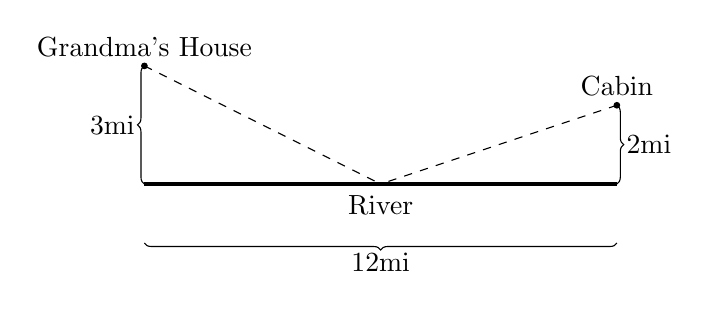
\begin{tikzpicture}
        \coordinate (A) at (0,1.5);
        \coordinate (B) at (6,1);
        \coordinate (C) at (3, 0);
        
        \filldraw[black] (A) circle (1pt) node[anchor=south] {Grandma's House};
        \filldraw[black] (B) circle (1pt) node[anchor=south] {Cabin};

        \draw[ultra thick] (0,0) -- node[anchor=north]{River} ++ (6,0);
        
        \draw[dashed] (A) -- (C);
        \draw[dashed] (B) -- (C);
        
        \draw[decorate,decoration={brace}]  (0,0) -- node[anchor=east]{3mi} ++ (A);
        \draw[decorate,decoration={brace, mirror}]  (6,0) -- node[anchor=west]{2mi} ++ (0,1);
        \draw[decorate,decoration={brace, mirror}]  (0,-.75) -- node[anchor=north]{12mi} ++ (6,0);
    \end{tikzpicture}
\end{center}

We can imagine reflecting Grandma's House across the River.

\begin{center}
    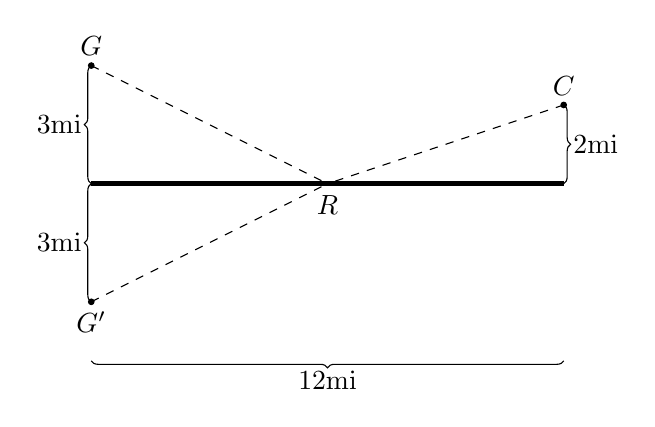
\begin{tikzpicture}
        \coordinate (A) at (0,1.5);
        \coordinate (B) at (6,1);
        \coordinate (C) at (3, 0);
        \coordinate (D) at (0, -1.5);
        
        \filldraw[black] (A) circle (1pt) node[anchor=south] {$G$};
        \filldraw[black] (B) circle (1pt) node[anchor=south] {$C$};
        \filldraw[black] (D) circle (1pt) node[anchor=north] {$G^\prime$};

        \draw[ultra thick] (0,0) -- node[anchor=north]{$R$} (6,0);
        
        \draw[dashed] (A) -- (C);
        \draw[dashed] (B) -- (C);
        
        \draw[dashed] (D) -- (C);
        
        \draw[decorate,decoration={brace}]  (0,0) -- node[anchor=east]{3mi} ++ (A);
        \draw[decorate,decoration={brace, mirror}]  (0,0) -- node[anchor=east]{3mi} ++ (D);
        \draw[decorate,decoration={brace, mirror}]  (6,0) -- node[anchor=west]{2mi} ++ (0,1);
        \draw[decorate,decoration={brace, mirror}]  (0,-2.25) -- node[anchor=north]{12mi} ++ (6,0);
    \end{tikzpicture}
\end{center}

Reflecting Grandma's house gives us a new path from $R$ to $G^\prime$, which has the same length as the path from $R$ to $G$. So if we find the shortest path $C$ to $R$ to $G^\prime$, it will have the same length as the shortest path $C$ to $R$ to $G^\prime$. The shortest path from $C$ to $G^\prime$ is a straight line passing through the river.

\begin{center}
    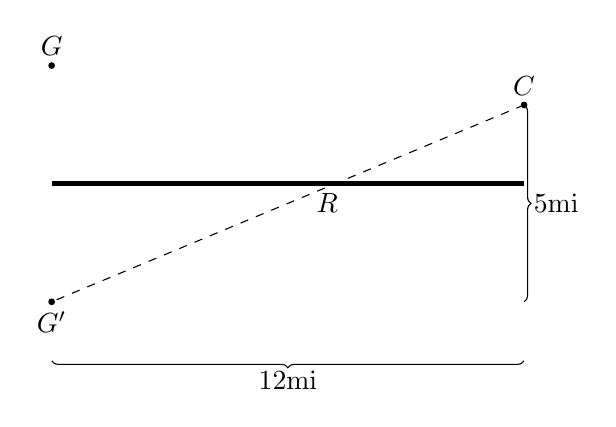
\begin{tikzpicture}
        \coordinate (A) at (0,1.5);
        \coordinate (B) at (6,1);
        \coordinate (C) at (3, 0);
        \coordinate (D) at (0, -1.5);
        
        \filldraw[black] (A) circle (1pt) node[anchor=south] {$G$};
        \filldraw[black] (B) circle (1pt) node[anchor=south] {$C$};
        \filldraw[black] (D) circle (1pt) node[anchor=north] {$G^\prime$};

        \draw[ultra thick] (0,0) --  (6,0);
        \draw (3.5,0) node[anchor=north]{$R$};

        \draw[dashed] (B) -- (D);
        
        \draw[decorate,decoration={brace}]  (6,1) -- node[anchor=west]{5mi} ++ (0,-2.5);
        \draw[decorate,decoration={brace, mirror}]  (0,-2.25) -- node[anchor=north]{12mi} ++ (6,0);
    \end{tikzpicture}
\end{center}

So our shortest path $C$ to $R$ to $G^\prime$ is the hypotenuse of a right triangle with leg lengths 5 and 12. Using the Pythagorean theorem,

\[\text{length} = \sqrt{5^2 + 12^2} = 13\]

So our shortest path $C$ to $R$ to $G$ is also 13 miles.


\section*{Problem 4}
\fbox{
    \parbox{\textwidth}{
        Find the length of the shortest path from the point (3,5) to the point (8,2) that touches the x-axis and also touches the y-axis
    }
}
\\

We'll say $A = (3,5)$ and $B = (8,2)$. Since our path must touch the $x$-axis and the $y$-axis, we can reflect $B$ and $A$ across each each axis, respectively to get $B^\prime$ and $A^\prime$.

\begin{center}
    \begin{tikzpicture}
        \draw[<->,ultra thick] (-2,0)--(5,0) node[right]{$x$};
        \draw[<->,ultra thick] (0,-2)--(0,3) node[above]{$y$};
        
        \filldraw[black] (1.5,2.5) circle (1pt) node[anchor=south] {$A$};
        \filldraw[black] (4,1) circle (1pt) node[anchor=west] {$B$};
        
        \filldraw[black] (-1.5,2.5) circle (1pt) node[anchor=south] {$A^\prime$};
        \filldraw[black] (4,-1) circle (1pt) node[anchor=west] {$B^\prime$};
        
        \draw[dashed] (-1.5,2.5) -- (4,-1);
    \end{tikzpicture}
\end{center}

The shortest path from $A^\prime$ to $B^\prime$ is the shown straight line. Using the Euclidean Distance Formula, we get

\[\text{length} = \sqrt{(8+3)^2 + (-2-5)^2} = \sqrt{170} = 13.0384...\]

Due to the symmetry of reflection, this is the same distance as the path from $A$ to $B$ touching both axes.


\section*{Problem 5}
\fbox{
    \parbox{\textwidth}{
         Given a point $(a, b)$ with $0 < b < a$, determine the minimum perimeter of a triangle with one vertex at $(a, b)$, one on the x-axis, and one on the line $y = x$. You may assume that a triangle of minimum perimeter exists.
    }
}
\\

We have the following.

\begin{center}
    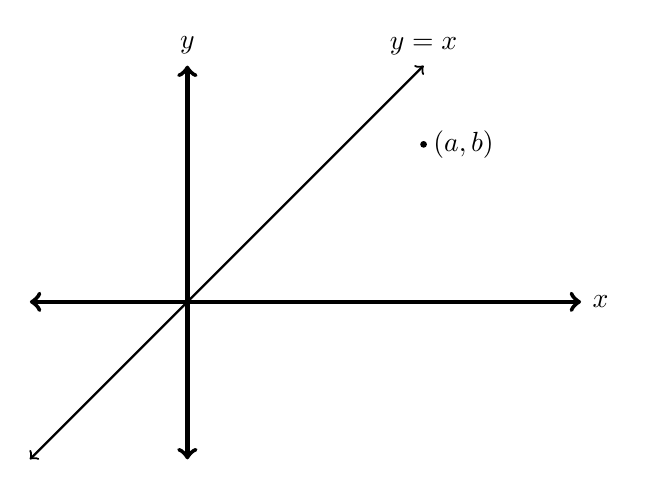
\begin{tikzpicture}
        \draw[<->,ultra thick] (-2,0)--(5,0) node[right]{$x$};
        \draw[<->,ultra thick] (0,-2)--(0,3) node[above]{$y$};
        \draw[<->,thick] (-2,-2)--(3,3) node[above]{$y=x$};
        
        \coordinate (a) at (3, 2);
         \filldraw[black] (a) circle (1pt) node[anchor=west] {$(a,b)$};
        
        
    \end{tikzpicture}
\end{center}

If we draw a line from $(a,b)$, touching $y=x$, and then to the x-axis, we get

\begin{center}
    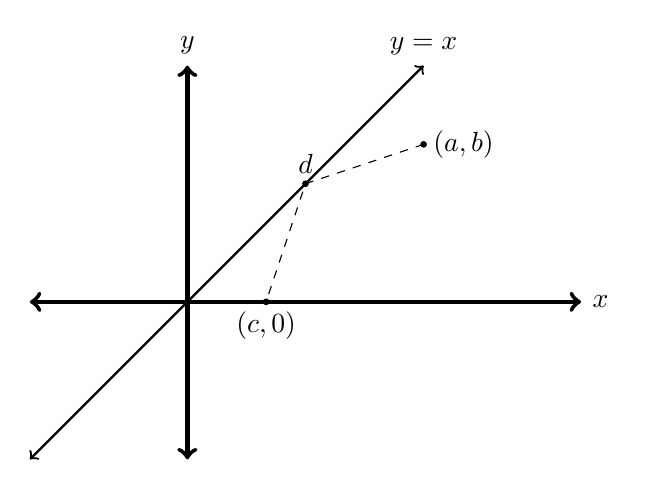
\begin{tikzpicture}
        \draw[<->,ultra thick] (-2,0)--(5,0) node[right]{$x$};
        \draw[<->,ultra thick] (0,-2)--(0,3) node[above]{$y$};
        \draw[<->,thick] (-2,-2)--(3,3) node[above]{$y=x$};
        
        \coordinate (a) at (3, 2);
        \coordinate (b) at (1.5, 1.5);
        \coordinate (c) at (1, 0);
        
        \filldraw[black] (a) circle (1pt) node[anchor=west] {$(a,b)$};
        \filldraw[black] (b) circle (1pt) node[anchor=south] {$d$};
        \filldraw[black] (c) circle (1pt) node[anchor=north] {$(c,0)$};
        
        \draw[dashed] (a) -- (b) -- (c);
        
        
    \end{tikzpicture}
\end{center}

If we reflect the lower segment across the line $y=x$, we get a segment of equal length.

\begin{center}
    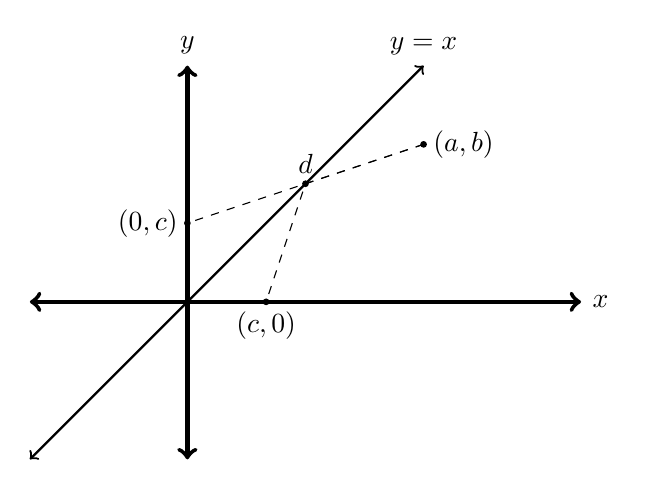
\begin{tikzpicture}
        \draw[<->,ultra thick] (-2,0)--(5,0) node[right]{$x$};
        \draw[<->,ultra thick] (0,-2)--(0,3) node[above]{$y$};
        \draw[<->,thick] (-2,-2)--(3,3) node[above]{$y=x$};
        
        \coordinate (a) at (3, 2);
        \coordinate (b) at (1.5, 1.5);
        \coordinate (c) at (1, 0);
        \coordinate (c2) at (0, 1);
        
        \filldraw[black] (a) circle (1pt) node[anchor=west] {$(a,b)$};
        \filldraw[black] (b) circle (1pt) node[anchor=south] {$d$};
        \filldraw[black] (c) circle (1pt) node[anchor=north] {$(c,0)$};
        \filldraw[black] (c2) circle (1pt) node[anchor=east] {$(0,c)$};
        
        \draw[dashed] (a) -- (b) -- (c);
        \draw[dashed] (a) -- (b) -- (c2);
        
        
    \end{tikzpicture}
\end{center}

Here, the clearly shortest path to the y-axis is a straight line so

\begin{center}
    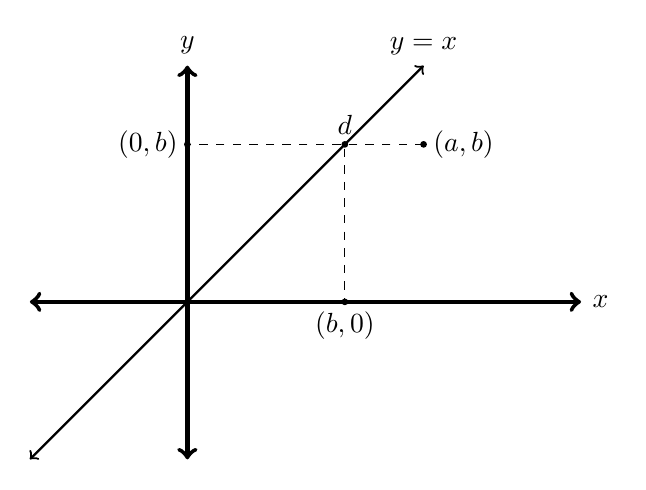
\begin{tikzpicture}
        \draw[<->,ultra thick] (-2,0)--(5,0) node[right]{$x$};
        \draw[<->,ultra thick] (0,-2)--(0,3) node[above]{$y$};
        \draw[<->,thick] (-2,-2)--(3,3) node[above]{$y=x$};
        
        \coordinate (a) at (3, 2);
        \coordinate (b) at (2, 2);
        \coordinate (c) at (2, 0);
        \coordinate (c2) at (0, 2);
        
        \filldraw[black] (a) circle (1pt) node[anchor=west] {$(a,b)$};
        \filldraw[black] (b) circle (1pt) node[anchor=south] {$d$};
        \filldraw[black] (c) circle (1pt) node[anchor=north] {$(b,0)$};
        \filldraw[black] (c2) circle (1pt) node[anchor=east] {$(0,b)$};
        
        \draw[dashed] (a) -- (b) -- (c);
        \draw[dashed] (a) -- (b) -- (c2);
        
        
    \end{tikzpicture}
\end{center}

Which is the shortest lengths for these two segments, and if we draw in a line connecting $(a,b)$ and $(c, 0)$ we will have our smallest perimeter triangle.

\begin{center}
    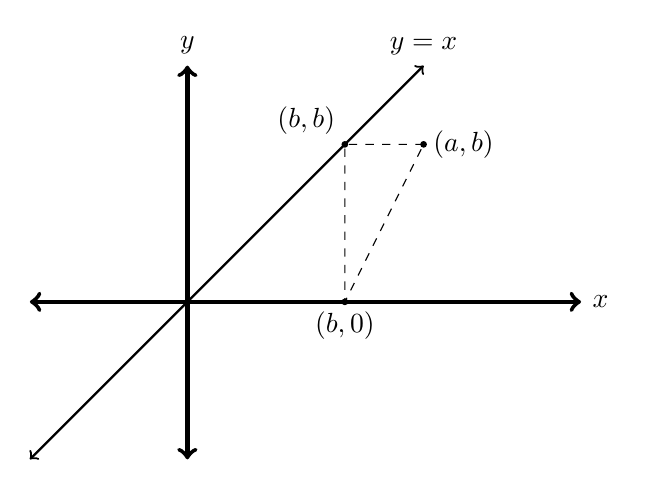
\begin{tikzpicture}
        \draw[<->,ultra thick] (-2,0)--(5,0) node[right]{$x$};
        \draw[<->,ultra thick] (0,-2)--(0,3) node[above]{$y$};
        \draw[<->,thick] (-2,-2)--(3,3) node[above]{$y=x$};
        
        \coordinate (a) at (3, 2);
        \coordinate (b) at (2, 2);
        \coordinate (c) at (2, 0);
        
        \filldraw[black] (a) circle (1pt) node[anchor=west] {$(a,b)$};
        \filldraw[black] (b) circle (1pt) node[anchor=south east] {$(b,b)$};
        \filldraw[black] (c) circle (1pt) node[anchor=north] {$(b,0)$};
        
        \draw[dashed] (a) -- (b) -- (c) -- (a);
        
        
    \end{tikzpicture}
\end{center}

So our side lengths are
\[b\]
\[a-b\]
\[\sqrt{b^2 + (a-b)^2} = \sqrt{a^2 - 2ab + 2b^2}\]

So our perimeter is
\[b + (a-b) + \sqrt{a^2 - 2ab + 2b^2}\]
\[a + \sqrt{a^2 - 2ab + 2b^2}\]


\newpage
\section*{Problem 6}
\fbox{
    \parbox{\textwidth}{
        Four bugs are situated at each vertex of a unit square. Suddenly, each bug begins to chase its counterclockwise neighbor. If the bugs travel at 1 unit per minute, how long will it take for the four bugs to crash into one another?
    }
}
\\
Since each bug starts in the corner of a square, at the moment they start chasing their neighbor, each of their desired movement directions is perpendicular to the bug they are chasing. As the situation continues, the bugs all move at the same speed, so there is always rotational symmetry between them. So each bugs desired direction is always perpendicular to the bug's they are chasing. So the bugs are always at the corners of a square that is shrinking. The bugs will collide in the center.

\begin{center}
    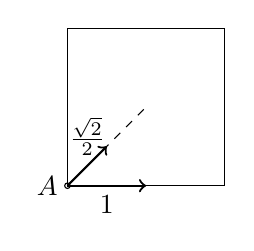
\begin{tikzpicture}
        \coordinate (A) at (0, 0);
        \coordinate (B) at (2, 0);
        \coordinate (C) at (2, 2);
        \coordinate (D) at (0, 2);
        
        \draw[black] (A) circle (1pt) node[anchor=east] {$A$};
        \draw[black] (A) -- (B) -- (C) -- (D) -- (A);
        
        \draw[->, thick, black] (A) -- node[anchor=north] {1} (1,0);
        \draw[->, thick, black] (A) -- node[anchor=south] {$\frac{\sqrt{2}}{2}$} (0.5,0.5);
        \draw[dashed] (A) -- (1,1);
    
    \end{tikzpicture}
\end{center}

The arrow towards the right represents bug $A$'s speed of 1 unit per minute towards its target bug. Since it is always part of a square in this way, the component of this speed towards the center, using a 45-degree right triangle is $\sqrt{2}/2$ units per minute. The original square is 1 unit by 1 unit, so the distance from a corner to the center is $\sqrt{2}/2$. Since the bugs travels this distance towards the center in 1 minute, they will all meet in the center after 1 minute.


\section*{Problem 7}
\fbox{
    \parbox{\textwidth}{
        Lockers in a row are numbered 1, 2, 3, ..., 1000. At first, all the lockers are closed. A person walks by and opens every other locker, starting with locker #2. Thus lockers 2, 4, 6, ..., 998, 1000 are open. Another person walks by, and changes the “state” (i.e., closes a locker if it is open, opens a locker if it is closed) of every third locker, starting with #3. Then another person changes the state of every fourth locker, starting with #4, etc. This process continues until no more lockers can be altered. Which lockers will be closed?
    }
}
\\

Each locker number will have its state swapped a number of times equal to it's number of factors, excluding 1. Factors of numbers come in factor pairs, this includes prime numbers(1 and itself). Because of this, every number has an even number of factors, except for perfect squares, because one of the factor pairs for a perfect square $n^2$ is $n$ and $n$.  Perfect squares thus have an odd number of factors. Since no lockers are flipped on 1, then all numbers will have it's state swapped an odd number of times, except for perfect squares, which will have their states swapped an even number of times. Since they all start closed, only the perfect square number lockers will be closed at the end.


\newpage
\section*{Problem 8}
\fbox{
    \parbox{\textwidth}{
        Take 15 coins and put them in an equilateral triangle touching each other. Show that independently on how they are placed, there must always be three coins, all three heads or all three tails, whose center form an equilateral triangle.
    }
}
\\

We have the following.

\begin{center}
    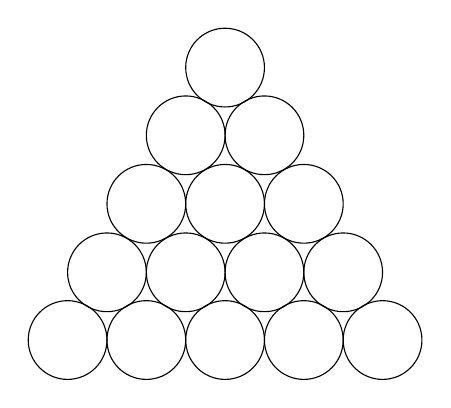
\begin{tikzpicture}
        \draw[black] (0,0) circle (0.5cm);
        \draw[black] (1,0) circle (0.5cm);
        \draw[black] (2,0) circle (0.5cm);
        \draw[black] (3,0) circle (0.5cm);
        \draw[black] (4,0) circle (0.5cm);
        
        \draw[black] (0.5,.86) circle (0.5cm);
        \draw[black] (1.5,.86) circle (0.5cm);
        \draw[black] (2.5,.86) circle (0.5cm);
        \draw[black] (3.5,.86) circle (0.5cm);
        
        \draw[black] (1,1.73) circle (0.5cm);
        \draw[black] (2,1.73) circle (0.5cm);
        \draw[black] (3,1.73) circle (0.5cm);
        
        \draw[black] (1.5,2.6) circle (0.5cm);
        \draw[black] (2.5,2.6) circle (0.5cm);
        
        \draw[black] (2,3.46) circle (0.5cm);
    \end{tikzpicture}
\end{center}

We'll show coins as distinctly black and white, interchangeable for heads or tails either way. So the following will And firstly, assume that it is possible to arrange the coins such that no three heads or three tails form an equilateral triangle.

We also see that every triangle of 15 coins contains a triangle of 10 coins which must also be able to be arranged without equilateral triangles.

\begin{center}
    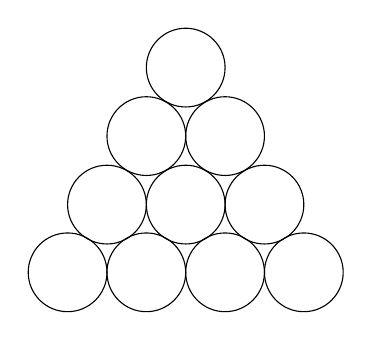
\begin{tikzpicture}
        \draw[black] (0,0) circle (0.5cm);
        \draw[black] (1,0) circle (0.5cm);
        \draw[black] (2,0) circle (0.5cm);
        \draw[black] (3,0) circle (0.5cm);
        
        \draw[black] (0.5,.86) circle (0.5cm);
        \draw[black] (1.5,.86) circle (0.5cm);
        \draw[black] (2.5,.86) circle (0.5cm);
        
        \draw[black] (1,1.73) circle (0.5cm);
        \draw[black] (2,1.73) circle (0.5cm);
        
        \draw[black] (1.5,2.6) circle (0.5cm);
        
    \end{tikzpicture}
\end{center}

We'll call the center coin black (recall this could also be done starting with white, it just matters they are distinct), and number the rest of the coins so they are easy to refer to.

\begin{center}
    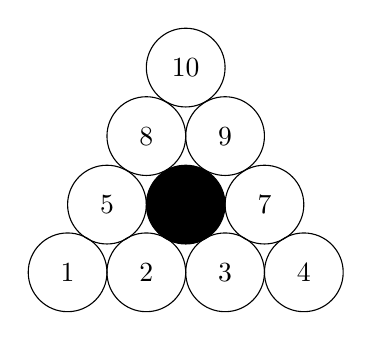
\begin{tikzpicture}
        \draw[black] (0,0) circle (0.5cm) node {1};
        \draw[black] (1,0) circle (0.5cm) node {2};
        \draw[black] (2,0) circle (0.5cm) node {3};
        \draw[black] (3,0) circle (0.5cm) node {4};
        
        \draw[black] (0.5,.86) circle (0.5cm) node {5};
        \filldraw[black] (1.5,.86) circle (0.5cm) node {6};
        \draw[black] (2.5,.86) circle (0.5cm) node {7};
        
        \draw[black] (1,1.73) circle (0.5cm) node {8};
        \draw[black] (2,1.73) circle (0.5cm) node {9};
        
        \draw[black] (1.5,2.6) circle (0.5cm) node {10};
        
    \end{tikzpicture}
\end{center}

Currently 3, 5, and 9 form an equilateral triangle of white coins, so one must be black. it doesn't matter which one we pick because each would be symmetrical to any other through rotation. We'll select 5.

\begin{center}
    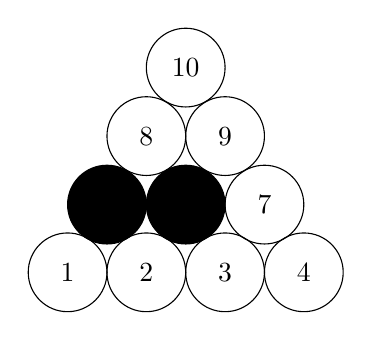
\begin{tikzpicture}
        \draw[black] (0,0) circle (0.5cm) node {1};
        \draw[black] (1,0) circle (0.5cm) node {2};
        \draw[black] (2,0) circle (0.5cm) node {3};
        \draw[black] (3,0) circle (0.5cm) node {4};
        
        \filldraw[black] (0.5,.86) circle (0.5cm) node {5};
        \filldraw[black] (1.5,.86) circle (0.5cm) node {6};
        \draw[black] (2.5,.86) circle (0.5cm) node {7};
        
        \draw[black] (1,1.73) circle (0.5cm) node {8};
        \draw[black] (2,1.73) circle (0.5cm) node {9};
        
        \draw[black] (1.5,2.6) circle (0.5cm) node {10};
        
    \end{tikzpicture}
\end{center}

Likewise for 2, 8, and 7. However, if we choose either 2 or 8, we would form a small equilateral triangle of black coins, so we must choose 7.

\begin{center}
    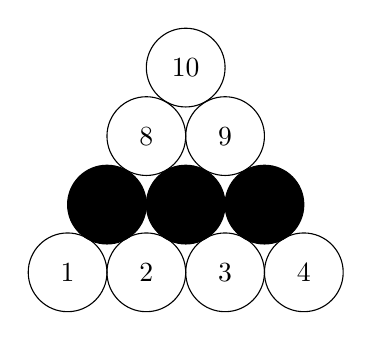
\begin{tikzpicture}
        \draw[black] (0,0) circle (0.5cm) node {1};
        \draw[black] (1,0) circle (0.5cm) node {2};
        \draw[black] (2,0) circle (0.5cm) node {3};
        \draw[black] (3,0) circle (0.5cm) node {4};
        
        \filldraw[black] (0.5,.86) circle (0.5cm) node {5};
        \filldraw[black] (1.5,.86) circle (0.5cm) node {6};
        \filldraw[black] (2.5,.86) circle (0.5cm) node {7};
        
        \draw[black] (1,1.73) circle (0.5cm) node {8};
        \draw[black] (2,1.73) circle (0.5cm) node {9};
        
        \draw[black] (1.5,2.6) circle (0.5cm) node {10};
        
    \end{tikzpicture}
\end{center}

If we look at 10, we can see it is currently forming an equilateral triangle with 8 and 9, so it must be black. However, if we made it black, it would for an equilateral triangle with 5 and 7. So it must be white. Therefore, 10 must be both black and white, which is a contradiction. Therefore, our assumption is false, and it is not possible to arrange our 15 coin triangle without creating equilateral triangles out of 3 equal-state coins.


\section*{Problem 9}
\fbox{
    \parbox{\textwidth}{
        Wilson’s Theorem: Prove that for all primes p,
            $(p - 1)! \equiv -1 (\mod p)$.
    }
}
\\

For $p=2$, this is trivial,

\[(2-1)! = 1! = 1 \equiv -1 (\mod 2)\]

So we'll show for some prime $p>2$. By the definition of Factorial, we know that 

\[(p-1)! = 1 \cdot 2 \cdot 3 \cdots (p-3) \cdot (p-2) \cdot (p-1)\]

We'll call each of the factors on the right hand side $a_i$.

\[(p-1)! = a_1 \cdot a_2 \cdot a_3 \cdots a_{p-3} \cdot a_{p-2} \cdot a_{p-1}\]

Since $p$ is prime, we know that for all $a_i$, gcd$(a_i, p) = 1$. Using B\'ezout's Identity, we know that there must be some $x,y \in \Z$ such that

\[a_ix + py = 1\]

Since $py$ is some integer multiple of $p$,

\[a_ix \equiv 1 (\text{mod}p)\]

Due to the properties of multiplication in mod, we can replace $x$ with its common residue in mod$p$, which is a number from 0 to $p-1$, and $x \not \equiv 0 \text{mod}p$. So we can replace $x$ with another $a_j$. So for all $a_i$, there exists another $a_j$ such that

\[a_ia_j \equiv 1 \pmod{p}\]

It should also be clear that that $a_i \equiv a_j \pmod{p}$ iff $a_i,a_j \equiv 1 \pmod{p}$ or\\ $a_i,a_j \equiv -1 \pmod{p}$. So for all other values, $a_i \not \equiv a_j$. We can also show that for every $a_i$, the corresponding $a_j$ is unique.

If we assume that $a_i$ has two values $m,n \in \Z$ and $m \not \equiv n$ such that 
\[a_im \equiv 1\pmod{p}\]
\[a_in \equiv 1\pmod{p}\]
we could then say
\[a_im \equiv a_in\pmod{p}\]

From Number Systems 120FN:
\begin{center}
   $ax \equiv ay \pmod{N}$ implies $x \equiv y \pmod{N}$ iff $\gcd(a, N)=1$ 
\end{center}


Since $\gcd(a_i,p)=1$, we know $m \equiv n\pmod{p}$, which is a contradiction. So each $a_i$(other than 1 and -1) has a unique $a_j$ which satisfies $a_ia_j \equiv 1 \pmod{p}$. Going back to our original equation,

\[(p-1)! = a_1 \cdot a_2 \cdot a_3 \cdots a_{p-3} \cdot a_{p-2} \cdot a_{p-1}\]
\[(p-1)! = 1 \cdot a_2 \cdot a_3 \cdots a_{p-3} \cdot a_{p-2} \cdot (p-1)\]
\[(p-1)! \equiv 1 \cdot a_2 \cdot a_3 \cdots a_{p-3} \cdot a_{p-2} \cdot (-1) \pmod{p}\]

Since $p$ is odd, and there are $p-1$ factors, there are an even number of factors. Excluding 1 and -1, we know that every value $a_i$ can be paired with a unique $a_j$ such that $a_ia_j \equiv 1 \pmod{p}$. So we can simplify to

\[(p-1)! \equiv 1 \cdot 1 \cdots 1 \cdot (-1) \pmod{p}\]
which gives us
\[(p-1)! \equiv -1 \pmod{p}\]


\newpage
\section*{Problem 10}
\fbox{
    \parbox{\textwidth}{
        Solve $x^4 + x^3 + x^2 + x + 1 = 0$
    }
}
\\

If we rewrite the equation as
\[1 + x + x^2 + x^3 + x^4 = 0\]
it is easy to see that this is a geometric series with $a_0 = 1$, $n=5$, and $r=x$. We can use the equation for sum of a geometric series
\[a_0\frac{1-r^n}{1-r}\]
to get
\[\frac{1-x^5}{1-x} = 0\]

For this to be true, we must have
\[1-x \ne 0\]
\[1-x^5 = 0\]
so
\[x^5 = 1\]

Since $x=1$ doesn't work, we need to find the complex solutions. Complex numbers can be written in polar form as
\[x = a + bi = r(\cos\theta +i\sin\theta)\]
and we need to find $\theta$ values for
\[x = \cos\theta + i\sin\theta\]
such that
\[x^5 = \cos(5\theta) +i\sin(5\theta) = 1\]

So we need $\theta$ values such that $5\theta$ is equivalent to 0. So we can have
\begin{align*}
    \theta &= \frac{2\pi}{5} & x &= \cos(\frac{2\pi}{5}) + i\sin(\frac{2\pi}{5})\\
    \theta &= \frac{4\pi}{5} & x &= \cos(\frac{4\pi}{5}) + i\sin(\frac{4\pi}{5})\\
    \theta &= \frac{6\pi}{5} & x &= \cos(\frac{6\pi}{5}) + i\sin(\frac{6\pi}{5})\\
    \theta &= \frac{8\pi}{5} & x &= \cos(\frac{8\pi}{5}) + i\sin(\frac{8\pi}{5})
\end{align*}


\newpage
\section*{Problem 11}
\fbox{
    \parbox{\textwidth}{
        Prove that
        \[(a + b)(b + c)(c + a) \geq 8abc\]
        is true for all positive numbers a, b and c, with equality only if $a = b = c$.
    }
}
\\

Given that $a,b,c$ are all greater than 0 and any number squared is greater than 0,

\[a(b-c)^2 + b(a-c)^2 + c(a-b)^2 > 0\]

Multiply both sides by $abc$.

\[\frac{(b-c)^2}{bc} + \frac{(a-c)^2}{ac} + \frac{(a-b)^2}{ab} > 0\]

Expand numerators.

\[\frac{b^2 - 2bc +c^2}{bc} + \frac{a^2 -2ac +c^2}{ac} + \frac{a^2 - 2ac + c^2}{ab} > 0\]

Pull out the center terms.

\[\frac{b^2+c^2}{bc} - 2  + \frac{a^2+c^2}{ac} - 2 + \frac{a^2 + c^2}{ab} - 2 > 0\]

Add 6 to both sides.

\[\frac{b^2+c^2}{bc} + \frac{a^2+c^2}{ac} + \frac{a^2 + c^2}{ab} > 6\]

Separate the fractions.

\[\frac{b}{c} + \frac{c}{b} + \frac{a}{c} + \frac{c}{a} + \frac{a}{b} + \frac{b}{a} > 6\]

Combine like numerators.

\[\frac{a(b+c)}{bc} + \frac{b(a+c)}{ac} + \frac{c(a+b)}{ab} > 6\]

Multiply both sides by $abc$.

\[a^2(b+c) + b^2(a+c) + c^2(a+b) > 6abc\]

Add $2abc$ to both sides.

\[a^2(b+c) + b^2(a+c) + c^2(a+b) +2abc > 8abc\]

Distribute.

\[a^2b + a^2c + 2abc + ab^2 + ac^2 + b^2c + bc^2 > 8abc\]

Factor.

\[(a+b)(b+c)(a+c) > 8abc\]

And if a=b=c=x

\[(x+x)(x+x)(x+x) = 8xxx\]
\[(2x)^3 = 8x^3\]
\[8x^3 = 8x^3\]


\end{document}